\documentclass[../main.tex]{subfiles}
\begin{document}
\chapter{Design and implementation}


\subsection{Intervention Policies}

Another key advantage of using CBMs is having access to 
run-time interventions, which is the idea of utilizing professionals
to modify incorrect concept predictions to improve the 
performance of the model, as illustrated in Figure~\ref{fig:cbm-interventions} For simplicity, we omit the
possibility of incorrect interventions, i.e. the scenario
where the professional misjudges and changes the concept prediction to be incorrect,
and assume that
all interventions modify the concepts correctly. Thus an intervention
can be defined as the following function, where
the predicted concepts $\hat{\mathbf{c}}$ and the true concepts $\mathbf{c}$ are interpolated
via the intervention vector $\bm{\mu}$, a multi-hot encoded vector.
\[I(\hat{\mathbf{c}}, \mathbf{c}, \bm{\mu}) = 
\bm{\mu} \; \mathbf{c} + (1 - \bm{\mu}) \; \hat{\mathbf{c}} \qquad \hat{\mathbf{c}}, \mathbf{c}, \bm{\mu} \in \{0, 1\}^k\]

\begin{figure}[!h]
    \centering
    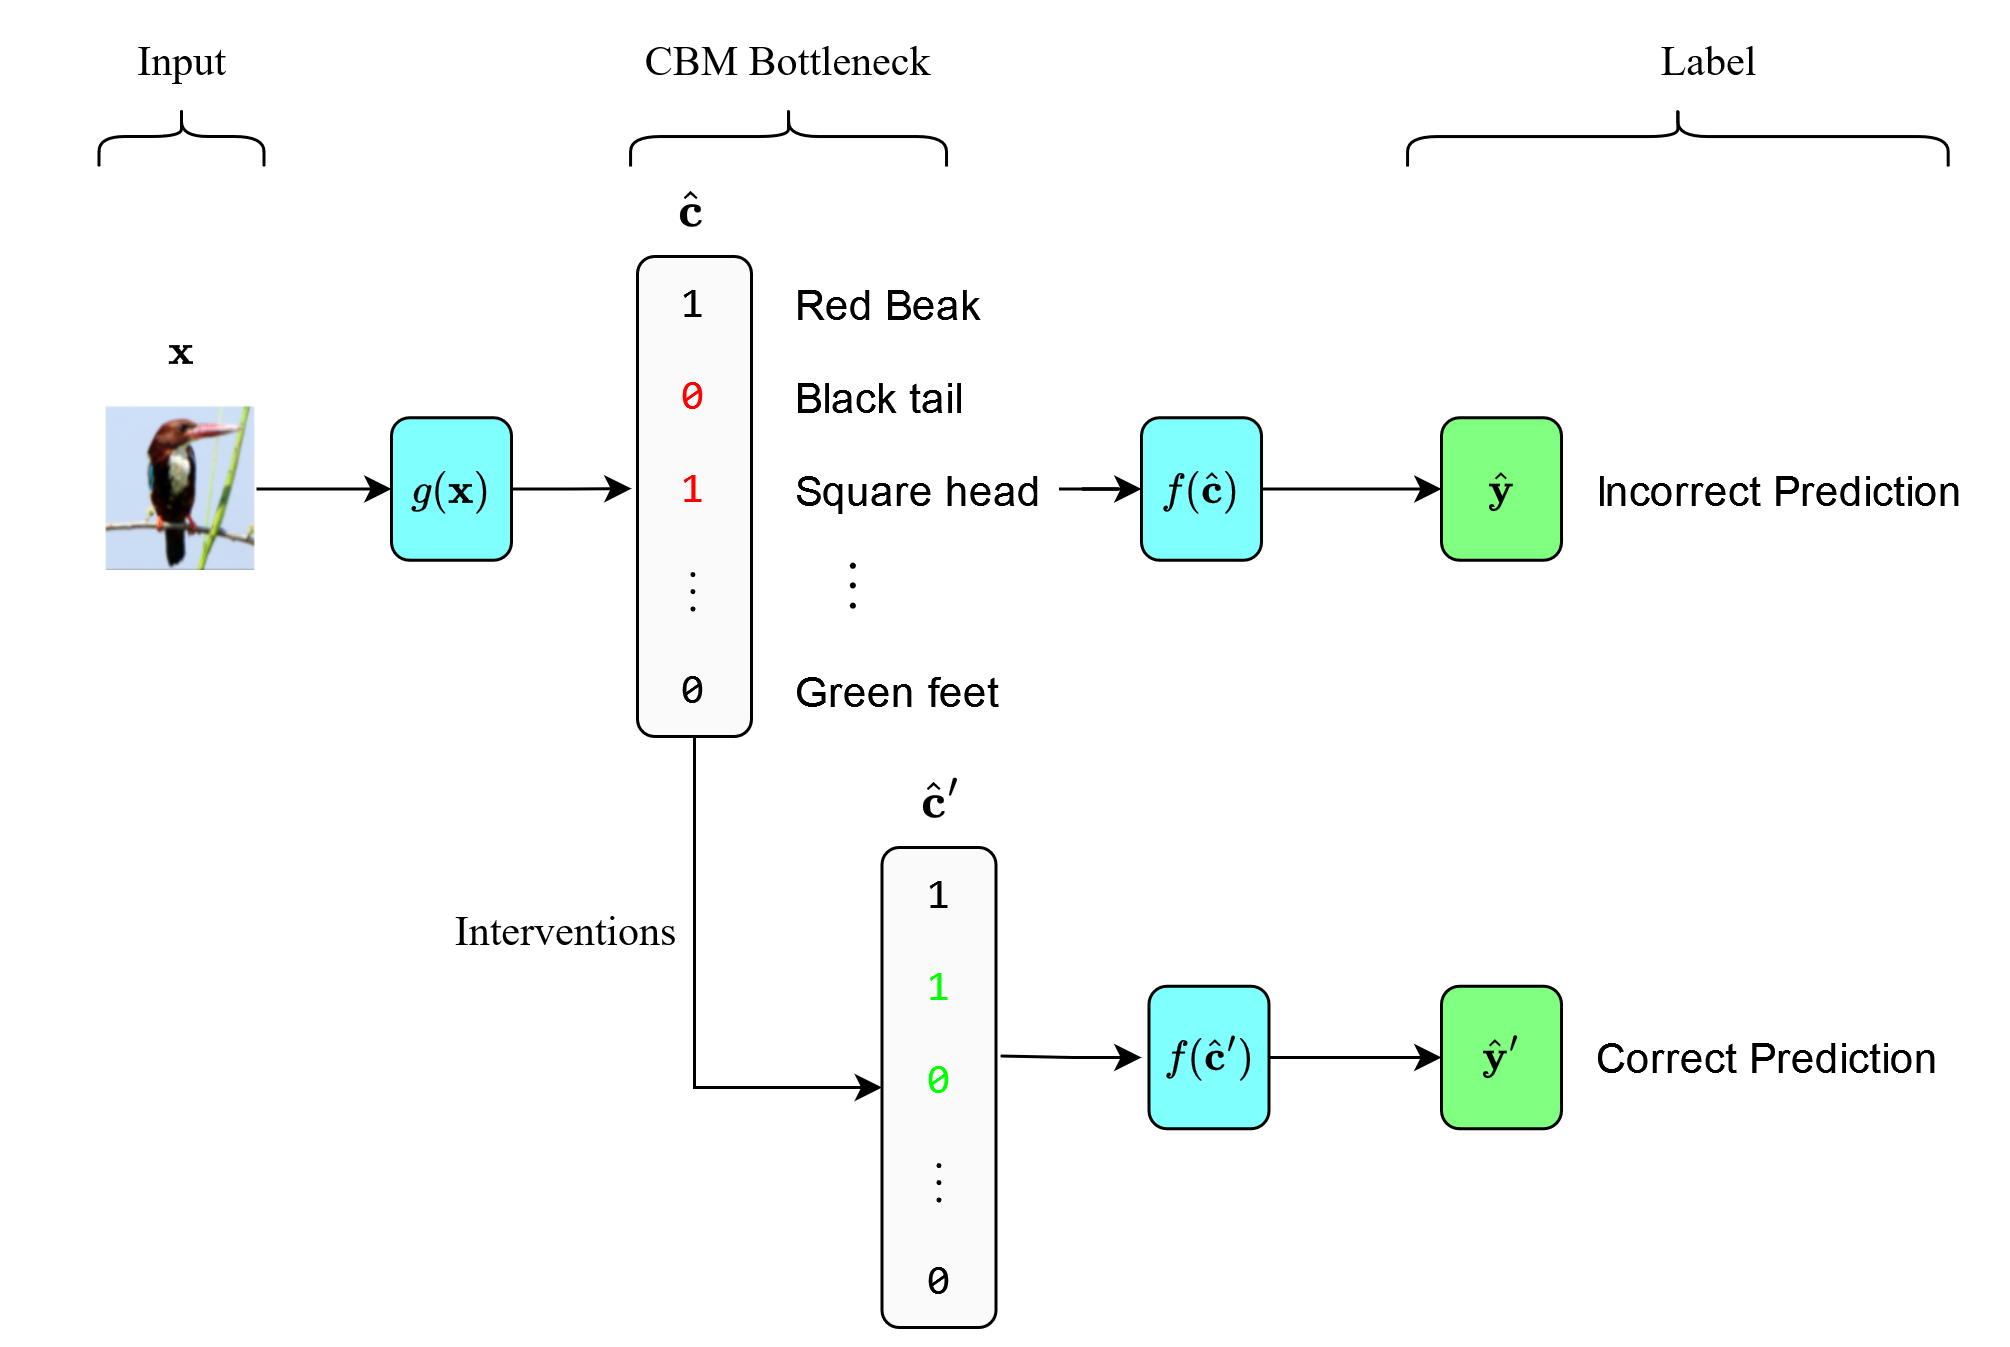
\includegraphics[width=\textwidth]{figs/background/cbm_interventions.png}
    \caption{An illustration of intervening on the concepts predicted by a CBM.}
    \label{fig:cbm-interventions}
\end{figure}

To formalize an intervention policy for this
project, we define an intervention policy $\mathcal{P}$ to be a policy, either learnt
or heuristic-based, that determines the order of concepts to intervene 
on with the goal of maximizing the performance after interventions.
If the performance of a model is measured by minimizing some loss $L_{\text{task}}$,
a greedy intervention policy is a collection of policies $\mathcal{P}_i$, each
outputting an index to intervene on at step $i$. The policy aims to minimizes 
the following:

\[\hat{\mathcal{P}} = \bigcup_{i=1}^k \mathop{\mathrm{argmin}}_{\mathcal{P}_i} L_{\text{task}}(\hat{g}(\hat{\mathbf{c}}_{\mathcal{P}_j}), \mathbf{y}) \]
% \[\hat{\mathcal{P}} = \mathop{\mathrm{argmin}}_{\mathcal{P}} \sum_{j = 1}^{k} L_{\text{task}}(\hat{g}(\hat{\mathbf{c}}_{\mathcal{P}, j}), \mathbf{y}) \]
\[\hat{\mathbf{c}}_{\mathcal{P}_0} = \hat{\mathbf{c}}, \hat{\mathbf{c}}_{\mathcal{P}_j} = I(\hat{\mathbf{c}}_{\mathcal{P}_{j-1}}, \mathbf{c}, \mathcal{P}_j(\hat{\mathbf{c}}_{\mathcal{P}_{j-1}}))\]
Which minimizes the loss at each step $j$ sequentially
for all $k$ concepts. At each
step, $\hat{\mathbf{c}}_{j-1}$ is 
the concept after the previous $j-1$ interventions,
Similar to above, the task loss $L_{\text{task}}$ is used to minimize
the discrepancy of $\hat{g}(\hat{\mathbf{c}}_{\mathcal{P}_j})$, 
the output of the label predictor model on the intervened concepts,
and label $\mathbf{y}$.

\subsection{Non-greedy Intervention Policies}


Compared to a greedy intervention policy, a non-greedy intervention 
policy outputs a set of concept to intervene on for a given budget $j$,
which we want to maximize the performance of the 
label predictor model on. This is equivalent to maximizing the following 
function:
\[\hat{\mathcal{P}} = \mathop{\mathrm{argmin}}_{\mathcal{P}} \sum_{j=1}^k L_{\text{task}}(\hat{g}(\hat{\mathbf{c}}_{\mathcal{P}_j}), \mathbf{y}) \]
\[\hat{\mathbf{c}}_{\mathcal{P}_j} = I(\hat{\mathbf{c}}, \mathbf{c}, \mathcal{P}(\hat{\mathbf{c}}, j))\]

Note that the notion of a budget, defined as the number
of concepts allowed to intervene on for simplicity, is only
important for non-greedy policies. Non-greedy policies aim
to maximize the performance after using up the intervention budget,
and may have a different set of intervention concepts 
for different budgets. Greedy policies always select the same
concepts per step and thus the current or remaining budget does not 
affect the concept selected by the policy.

We model the problem of finding a non-greedy intervention policy as a 
Reinforcement Learning problem. As mentioned in Section~\cite{background:rl},
Reinforcement Learning can be used to find non-greedy solutions to problems
by design as it models the long-term effects of its actions, and aims to 
maximize the overall reward gain 


\section{Surrogate Models}

We use surrogate models to model the probabilities of concepts which are used
to guide the RL model. Following Li et al.~\cite{afa} which uses Reinforcement Learning
in the similar problem of Active Feature Acquisition, we use a surrogate model to model
the conditional probabilities $p(\mathbf{x}_u \mid \mathbf{x}_o, \mathbf{y})$, 
where $\mathbf{x}_u$ is the set of unintervened concepts, $\mathbf{x}_o$ is the set of intervened concepts,
and $\mathbf{y}$ is the label. The surrogate model used is the Arbitrary Conditional Flow (AC Flow)~\cite{acflow}
model, which are flow-based models augmented with the power to model arbitrary conditional probabilities.

Flow-based models model probability distributions by leveraging the change of variable property~\cite{flow}.


\section{RLCEM}\label{method:rlcem}

\section{Datasets}
\end{document}